\chapter{Testing and Analysis}

\section{The Optically Thin Case}

\subsection{Finding an Appropriate Opening Angle}
\label{sec:bangForBuck}
For this test we used a $64^3$ particle glass (see \citet{wadsley2017}) of source particles with an equivalent but rotated glass of sink particles to produce a well mixed system of sinks and sources. This was then perturbed using the sum of 24 sinusoidal modes, as shown in equation \ref{eqn:sinemodes},
\begin{equation}
    \label{eqn:sinemodes}
    \overrightarrow{r} = \overrightarrow{r_0} + \sum_{i=1}^{24} \frac{1}{275} \sin(k_{x,i}r_x + k_{y,i}r_y + k_{z,i}r_z + \phi_i).
\end{equation}
The wavevector components, $k_i$, are are in the range [-5, 5] and the $\phi_i$ terms are in the range [0, 2$\pi$] and assign random phases to each mode. The constant in front of the sine was selected to limit the amplitude of the density perturbations created by these modes to within reasonable bounds \citep{grond}.

The system was run with opening angles varying between 0.1 and 1 and the RMS error relative to an opening angle of 0 of each gas particle's flux was calculated. At the same time, the number of rays traced per sink was logged, giving us an indicator of the computational cost of each opening angle. Plots of both of these values against opening angle are shown in \ref{fig:openingTest}
\begin{figure} [H]
    \centering
    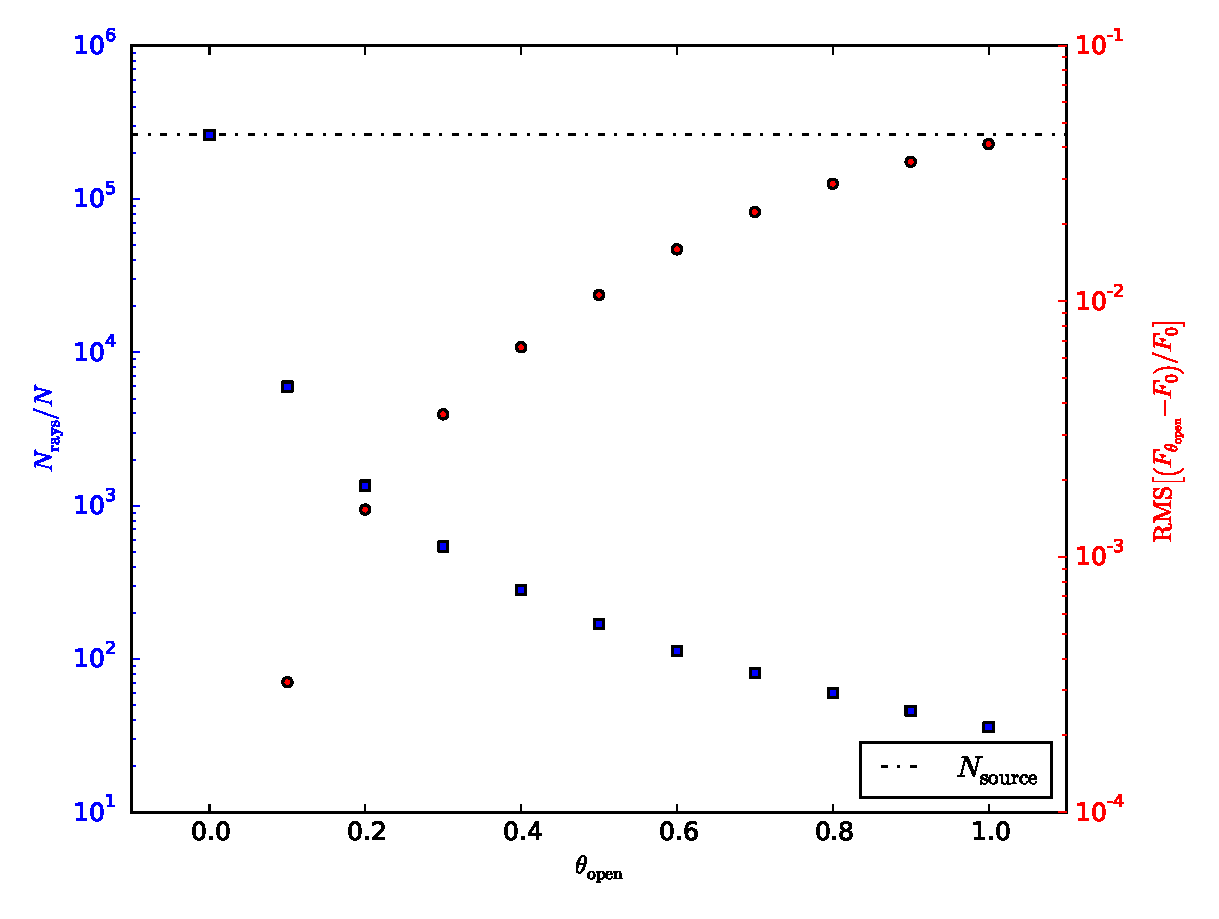
\includegraphics[width=\textwidth]{plots/CH4/opening_angle.pdf}
    \caption{RMS error and rays traced per sink for opening angles between 0 and 1.0}
    \label{fig:openingTest}
\end{figure}
After examining this plot, it was decided that we would use an opening angle of 0.5. This gives an RMS error of approximately $10^{-2}$ and a speedup of approximately $10^3$, i.e. requiring 0.1\% of the rays traced in the fully refined case. While this gives a good estimate of the appropriate opening angle for a well mixed system, simulations with dissimilar initial conditions may have differing optimal opening angles. These systems may benefit from repeating this test with ``toy" simulations that more closely approximate the system to find appropriate values for $\theta_{open}$. While testing the full simulation is possible, the time required to perform a full refinement test on a large system may make this challenging.

\subsection{Confirming Correct Scaling for Source Walk}

As the optically thin radiation algorithm is identical to that of gravity except for the force calculation, the scaling is identical at $\mathcal{O}(N_{sink} \log(N_{source}))$, as proven in \citet{grond}. To test this we used an identical initial condition to the previous test and changed the value of the opening angle from 0, giving full refinement, to an arbitrarily large value leading to no refinement. These are then compared to the minimum scaling of $\mathcal{O}(N_{sink} \log_2(N_{source}))$ and maximum scaling of $\mathcal{O}(N^2)$ in Figure \ref{fig:scalingThin}.

It can be seen that even a lower value of $\theta$ such as 0.4 still gives a substantial scaling improvement when compared to the full refinement, with ray counts up to nearly 3 orders of magnitude lower than that of the $\theta = 0$ test.
\begin{figure} [H]
    \centering
    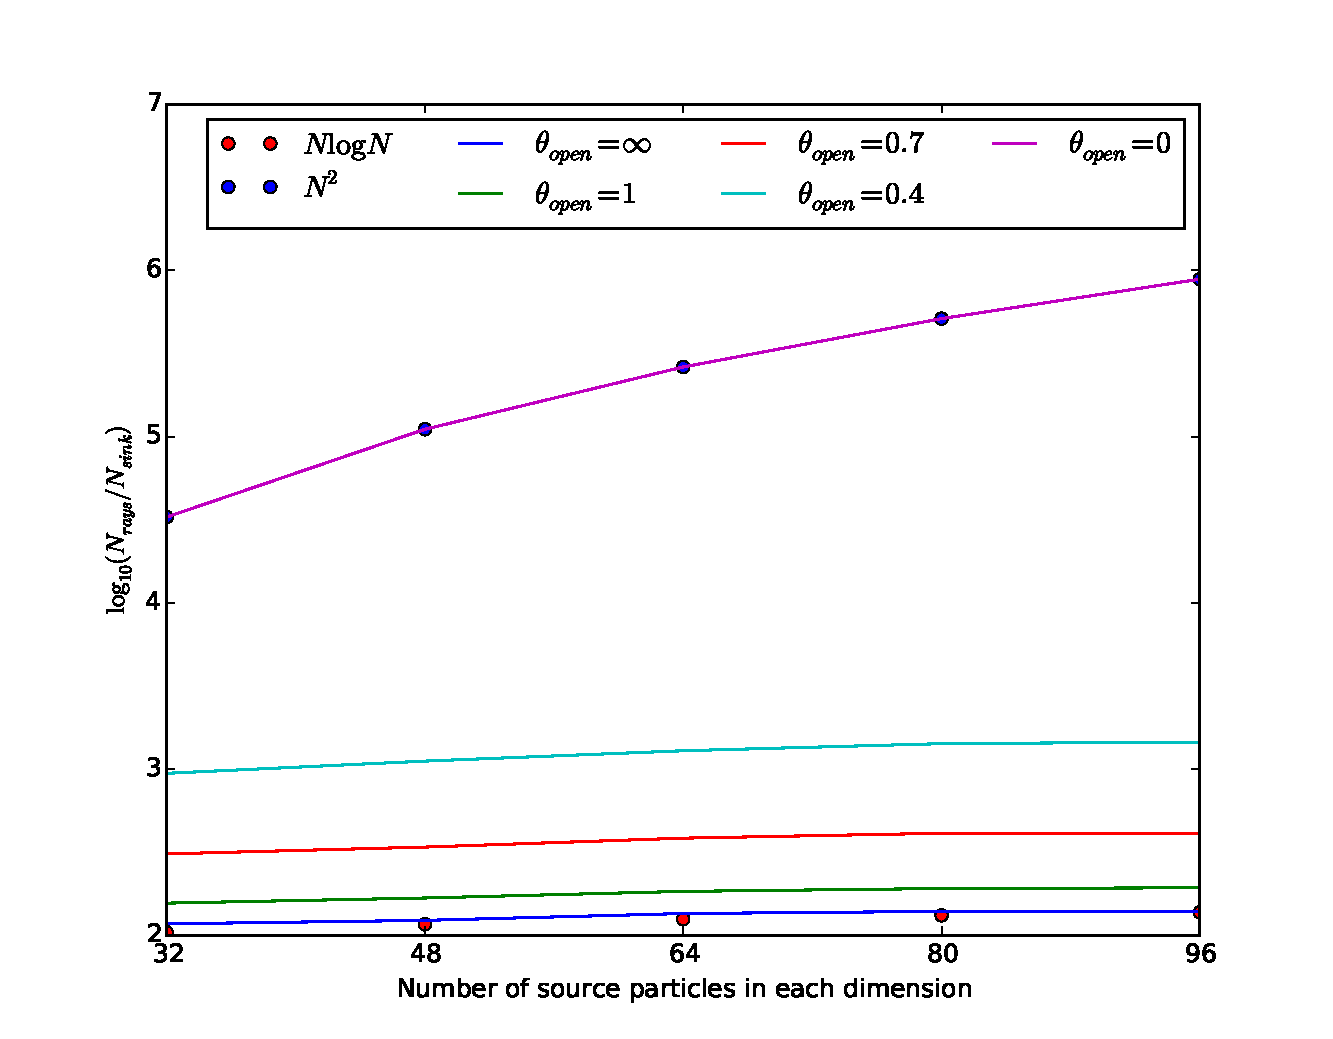
\includegraphics[width=\textwidth]{plots/CH4/scalingThin.pdf}
    \caption{Scaling of the optically thin (i.e. source walk) code. This is equivalent to that of the gravity walk}
    \label{fig:scalingThin}
\end{figure}
\subsection{Simulating Background Sources}

Some simulations require the creation of background sources to model such things as the cosmic ultraviolet background radiation. This can be approximated through the use of a sphere of background sources located at a great enough distance from the region of the simulation of interest with a luminosity that gives the required flux at the origin. This luminosity for each background source can be calculated by rearranging equation \ref{eqn:flux} in terms of L and dividing by the number of background particles, giving,

\begin{equation}
    L = \frac{4\pi r_{bg} F_{centre}}{N_{bg}},
\end{equation}

where $r_{bg}$, $F_{centre}$ and $N_{bg}$ are the radius of the background sphere, the expected flux in the centre of the system and the number of background particles respectively. 

Figure \ref{Fig:bgSource} shows the flux as a function of radius for a background source sphere at distance 0.5 from the simulation centre and an expected central flux of 1.0. It can be seen that the flux rapidly approaches the expected value of 1.0 with errors of only a few percent as far out as 0.2 from the centre. This implies that a reasonable proportion ($\sim 40 \%$) of the space contained by the background sources can be used for the simulation with minimal error in flux.

\begin{figure} [H]
    \centering
    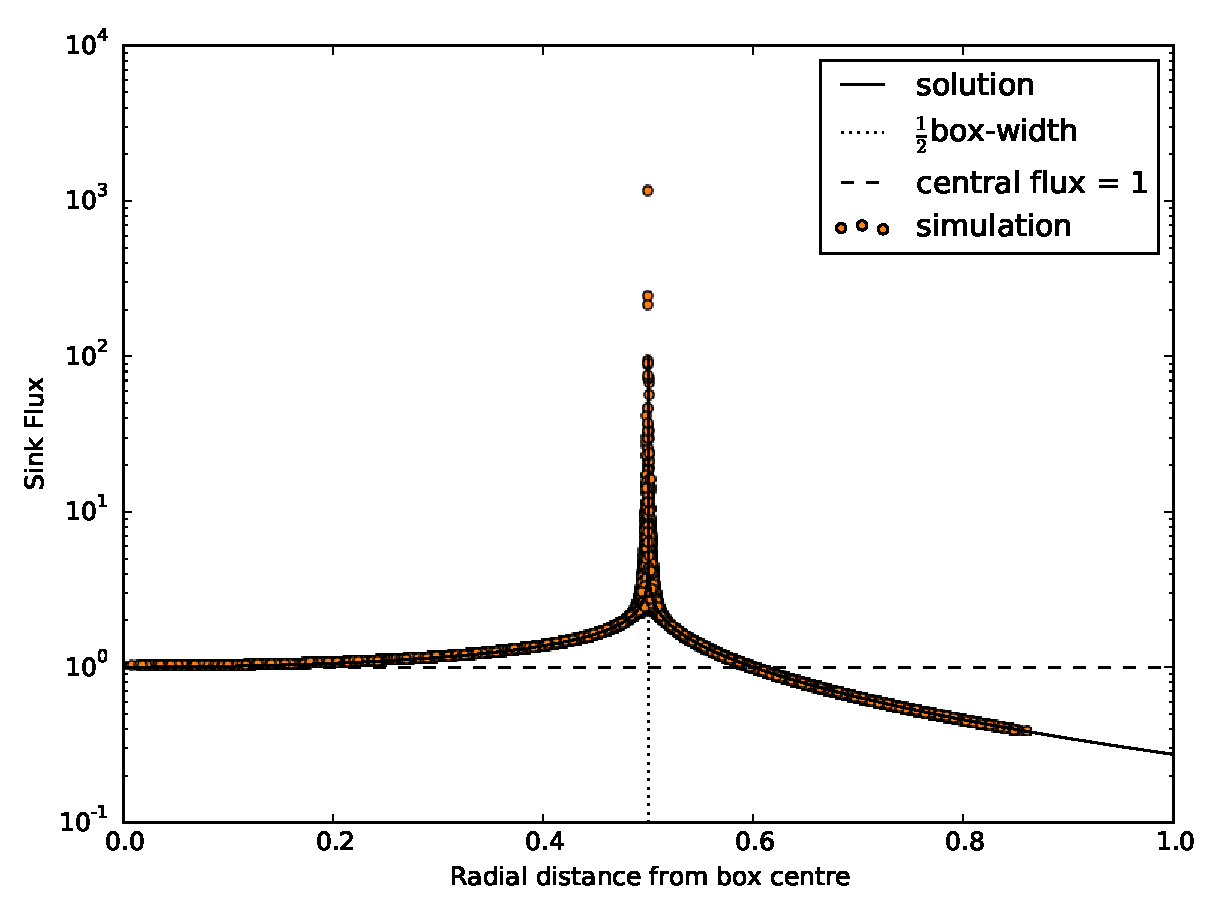
\includegraphics[width=0.7\textwidth]{plots/CH4/resultsCha.pdf}
    \caption{Flux against radial distance of background sources with total central flux of 1.0}
    \label{Fig:bgSource}
\end{figure}
    
\section{The Optically Thick Case}

\subsection{Uniform field test}
As an overall test of the accuracy of the optically thick code, we created a uniform gas field with 16 particles along each dimension whose optical depth across the box is 1, placed a star at the centre and measured the flux as a function of distance. As the absorption coefficient of this system is 1 in all space, the optical depth is exactly equal to the radial distance from the source, $r$. Thus, the simulated results can be compared to the analytical solution given in equation \ref{eqn:fluxUniform} to confirm that the optically thick code is functioning as expected,
\begin{equation}
    F = \frac{e^{-r}}{4\pi r^2}.
    \label{eqn:fluxUniform}
\end{equation}
Figure \ref{fig:uniformField} shows the results of this test, with the simulated results fitting near perfectly to the theoretical results.

\begin{figure} [H]
    \centering
    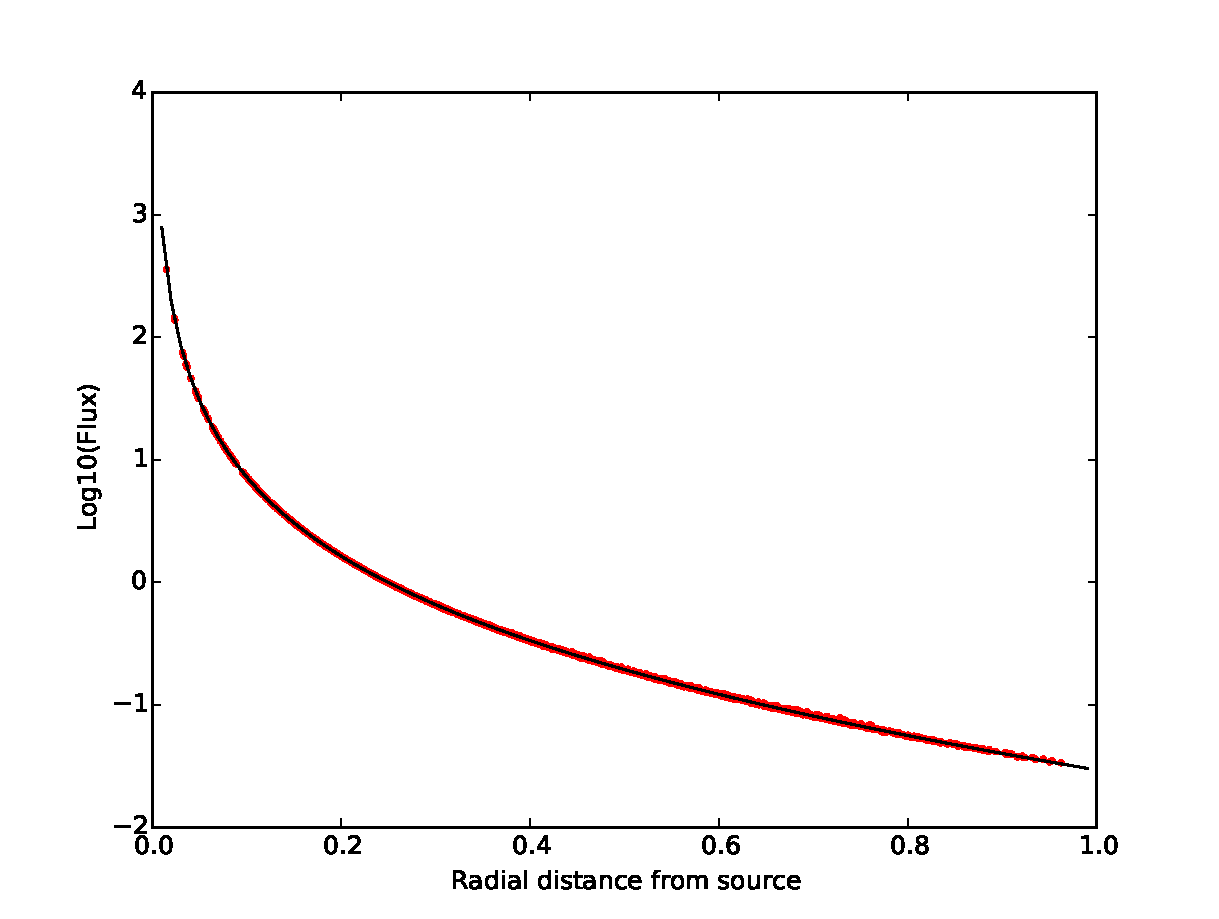
\includegraphics[width=\textwidth]{plots/CH4/thickFluxVr.pdf}
    \caption{Flux as a function of radius for a uniform density gas field compared to the analytic solution}
    \label{fig:uniformField}
\end{figure}

\subsection{Finding an Appropriate Maximum $\tau_{refine}$ Differential}

Finding an appropriate value for $\tau_{refine}$ can be done much the same way as finding the value for the opening angle, by changing its value and looking at both the speedup and the error. Unlike with the opening angle where we compared the number of rays, we instead compared the number of segments for all rays. 
\begin{figure} [H]
    \centering
    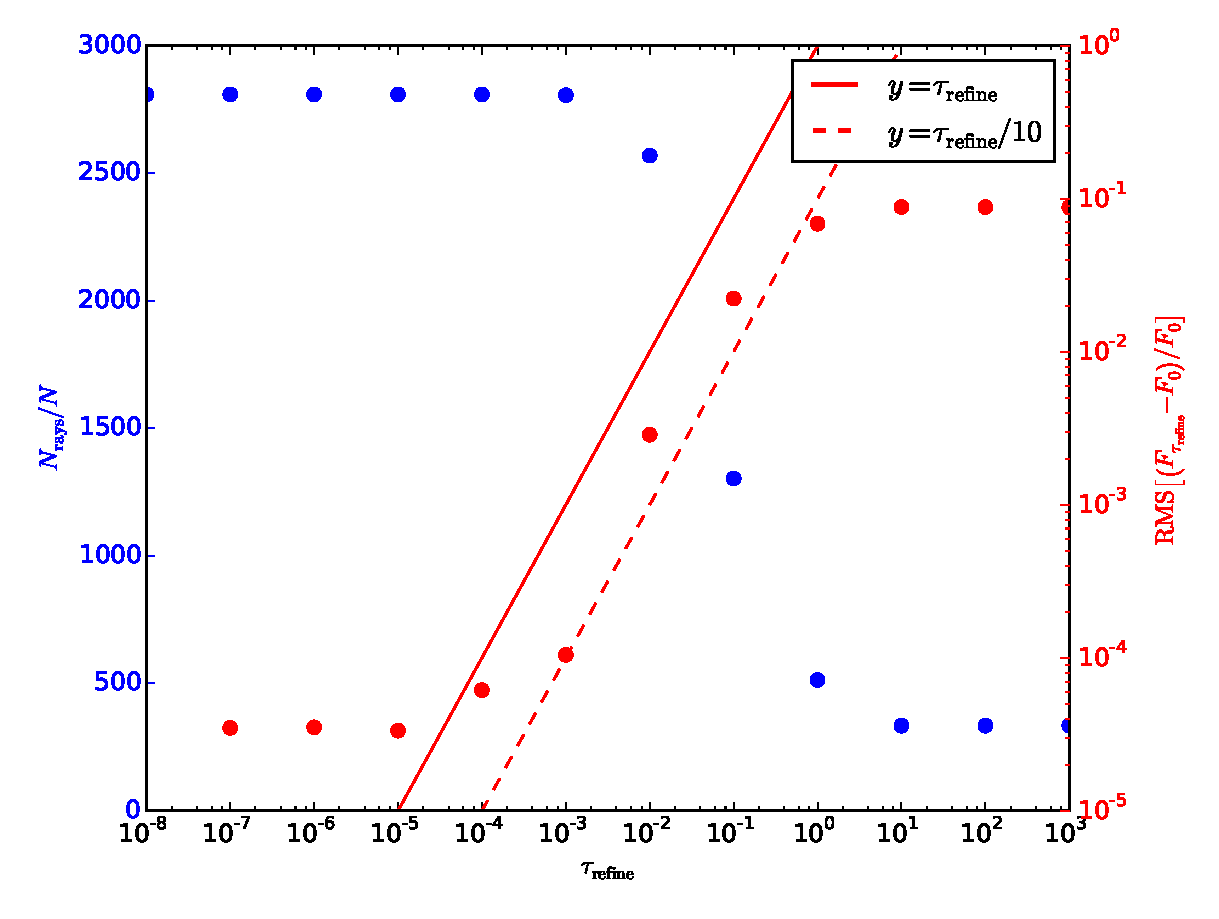
\includegraphics[width=\textwidth]{plots/CH4/tau_refine.pdf}
    \caption{Error in flux against maximum difference in $\tau$ of child nodes}
    \label{fig:maxTau}
\end{figure}
 The plateaus at both the lower and higher values of $\tau_{refine}$ are due to the limitations of refinement. For the lower values, this is caused by all values below $\tau_{refine} = 10^{-4}$ using purely bucket-scale absorption and for the higher values, only the P-P refinement criterion is being activated as the root node's $\tau$ perturbation is within permitted bounds. The two lines on Fig \ref{fig:maxTau} show the lines where the error is equivalent to $\tau_{refine}$ and $\tau_{refine}/10$. It can be seen that between refinement criterion values of $10^{-1}$ and $10^{-4}$, the error lies within these two lines, suggesting that the error in the absorption calculation is within an order of magnitude of the selected refinement criterion value. As there is no benefit to using a value of $\tau_{refine}$ lower than $10^{-3}$, optimal $\tau_{refine}$ was chosen to be between 0.1 and 0.01, depending on the accuracy required.

\subsection{Optically Thick Scaling Test}
To test the scaling of the Optically Thick code we once again ran simulations with increasing numbers of sinks and sources whose initial conditions are identical to that of the optically thin tests. The value of $\tau_{refine}$ was varied from 0.01 to an arbitrarily high value, i.e. no refinement, giving the results shown in Figure \ref{fig:scalingThick}. We chose 0.01 as the upper limit due to time constraints preventing us from running this test at full refinement.
\begin{figure} [H]
    \centering
    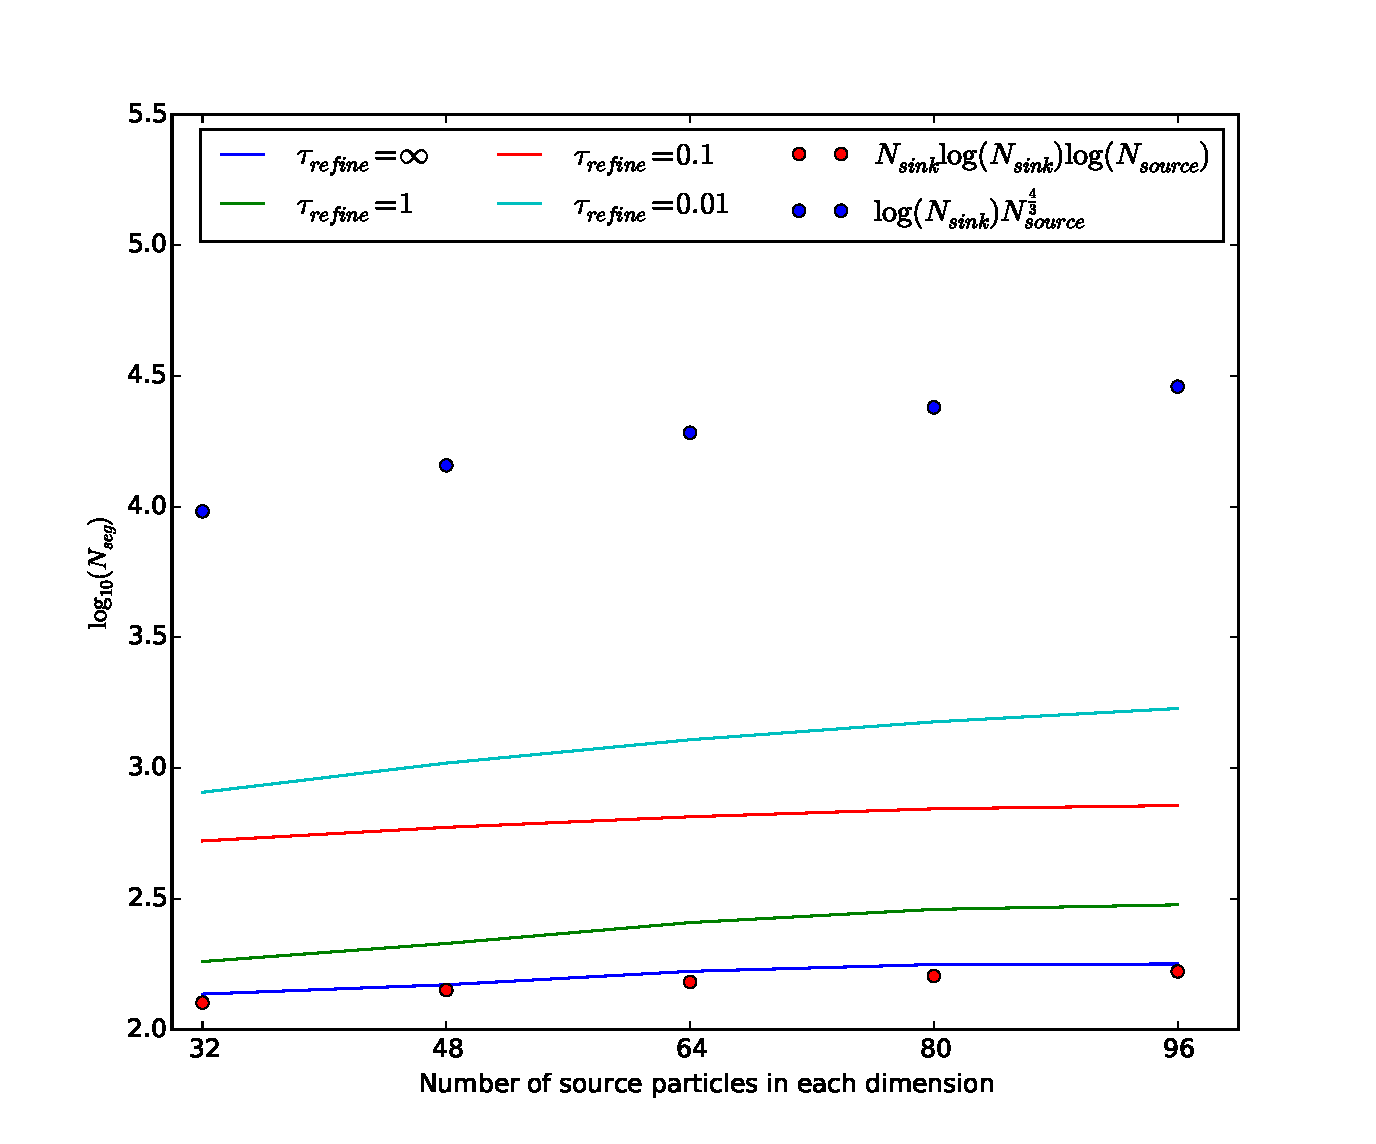
\includegraphics[width=\textwidth]{plots/CH4/tau_scaling.pdf}
    \caption{Scaling of the optically thick code.}
    \label{fig:scalingThick}
\end{figure}
The dotted values in Fig \ref{fig:scalingThick} show the minimum ($\mathcal{O}(N_{sink}\log{N_{sink}}\log{N_{source}})$) and maximum ($\mathcal{O}(N_{sink}^{\frac{4}{3}}\log{N_{source}})$) theoretical scaling. This maximum takes into account the reduction in computational cost from the source merging. Without this, the worst case scaling would be $\mathcal{O}(N_{source}N_{sink}^{\frac{4}{3}})$. It can be seen that the zero refinement case matches closely to the theoretical results and even lower values for the optically thick refinement parameter give strong scaling, with only a factor of 10 increase in the number of computations required.

\subsection{Isothermal Spheres test}

The isothermal spheres test was created to study the code's ability to create accurate shadows, regions where the flux from a source is blocked by dense objects. Multiple spheres whose densities follow a $\frac{1}{r}$ profile were created and placed with equal separation on the x = 0, z = 0 line. The source was placed at [-0.5, 0.4, 0], causing shadows behind the spheres with varying angular directions. 
\begin{figure} [H]
    \centering
    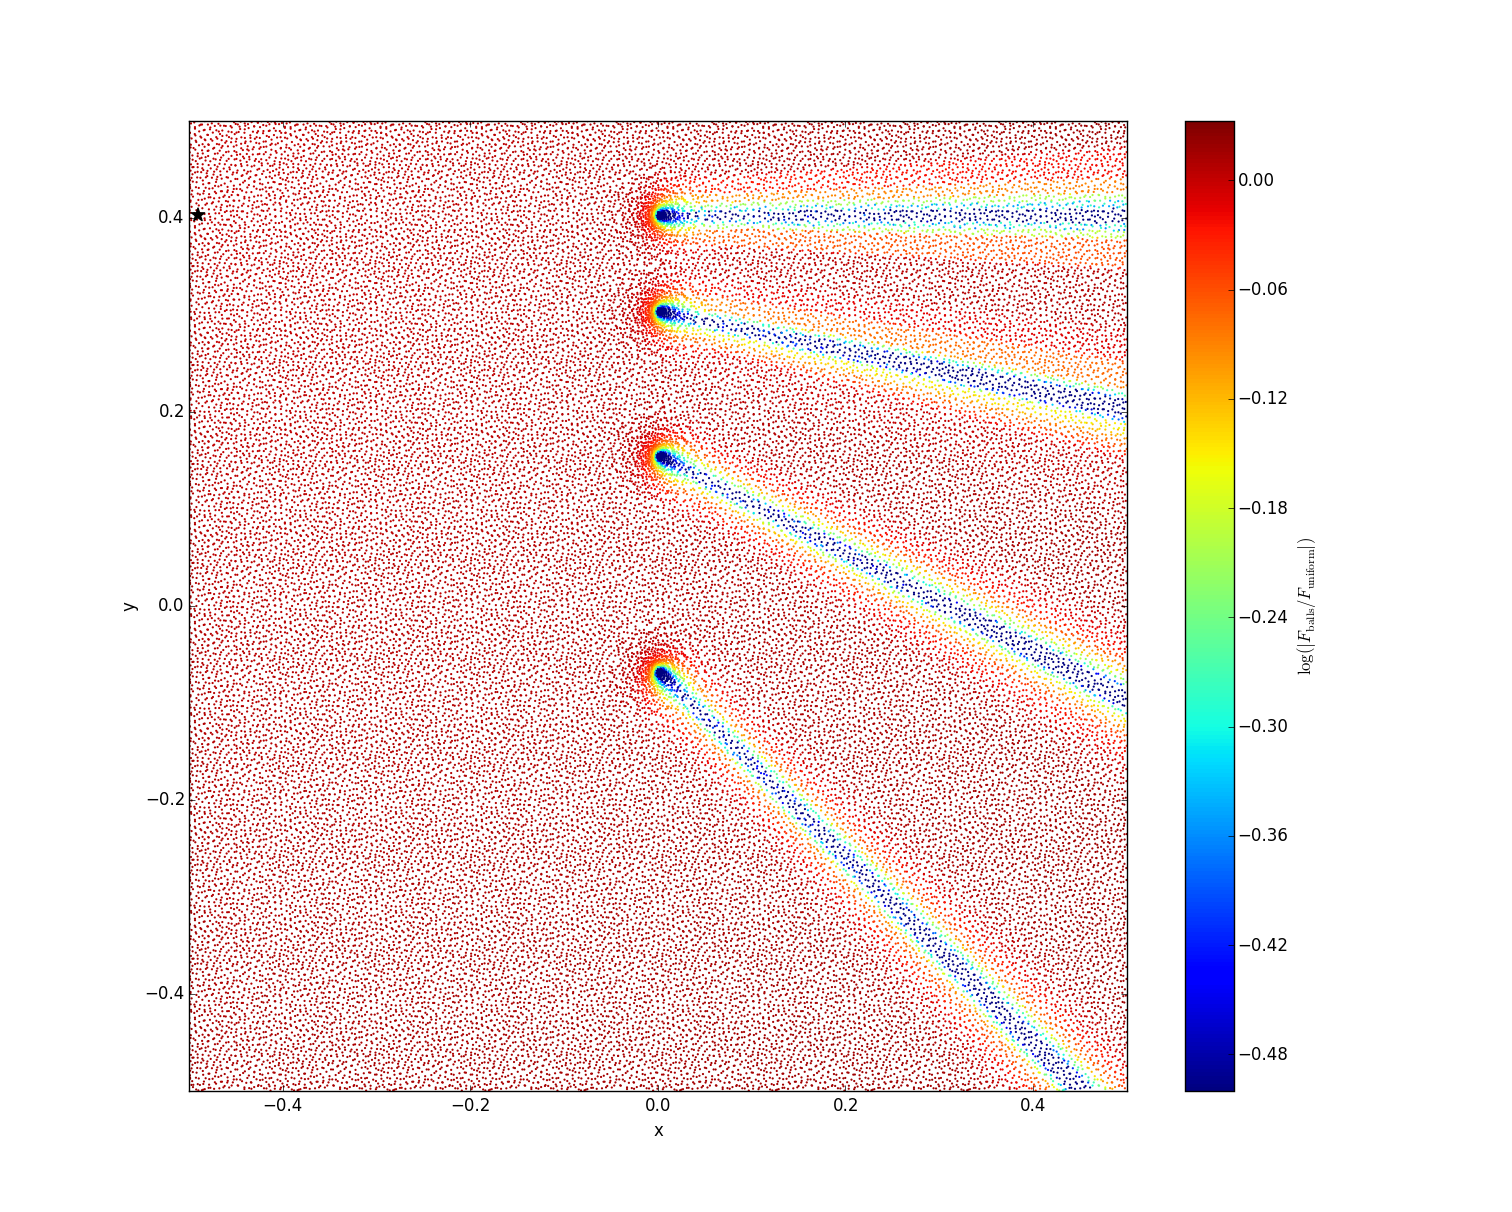
\includegraphics[width=\textwidth]{plots/CH4/balls_cha.png}
    \caption{Flux as a function of position of a uniform density gas with embedded isometric spheres. The data is normalized against the expected flux for an optical depth across the box of 1.0.}
    \label{fig:isoSpheres}
\end{figure}

The results for this test are comparable to those given in \citet{grond} where the errors are analyzed in detail.

\chapter{Complex sources}
\label{sec:complexsources}
The current refinement criterion for the source walk mimics that of gravity, where the only parameters that are used to determine whether a node should be opened or walked are the position and size of its bounding box. While this poses no issue when working with optically thin systems, when optically thick systems are treated the same way substantial error can arise. By moving the position of the sources in the node, we change the direction and dimensions of the ray walked between the sink and source and thus change the absorbing material intersected by the ray. Steps must be taken to make sure that any error introduced by source merging does not substantially alter the calculated flux and that the properties and distribution of the absorbing material are taken into account when selecting appropriate sources to perform ray tracing upon.

\section{Angular Dependence of Flux}
When sources are merged, the change in distance between each source and the sink at their initial, unmerged and their final, merged positions depend on the angle between the sink and source  node. This angle isn't taken into account when determining if a node should be opened and thus creates an error that is dependent on the angle on which the system is observed. For the optically thin case, these errors are second order and oscillate around zero with only a weak systematic bias. For randomly oriented source pairs there would be no systematic bias.

This can be shown by studying a system with two sources embedded inside a dense sphere, with each source an equal distance from the spheres centre. By taking measurements of the flux from both the combined and uncombined sources along a circle centred on the sphere and with a radius larger than the sphere radius we can see the error created by source merging. Figure \ref{fig:CSIC} shows the setup used to test this issue, with a sphere of radius 2, selected to represent a distance where source merging would occur, and sources embedded at a distance of 0.5 along the x-axis, either side of the sphere's centre. 
\begin{figure} [H]
    \centering
    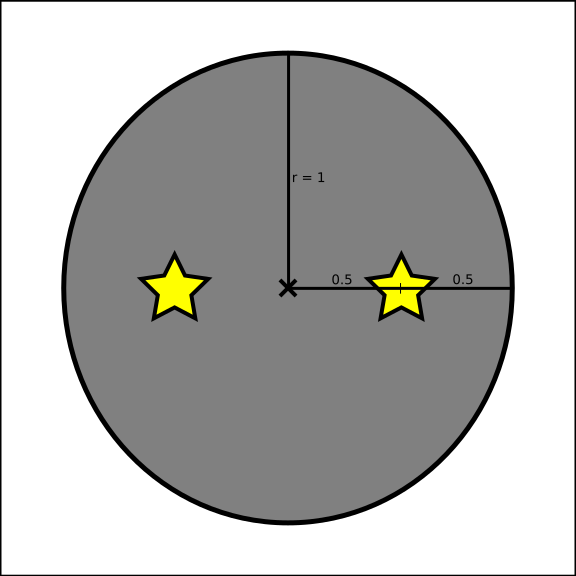
\includegraphics[width=\textwidth]{plots/CH4/CSICs.png}
    \caption{System setup for the angular dependence test}
    \label{fig:CSIC}
\end{figure}
The optical depth along the radius of the sphere was varied from 0 to 16, giving the error of the merged sources as a function of angle, shown in figure \ref{fig:CSAngular}.

\begin{figure} [H]
    \centering
    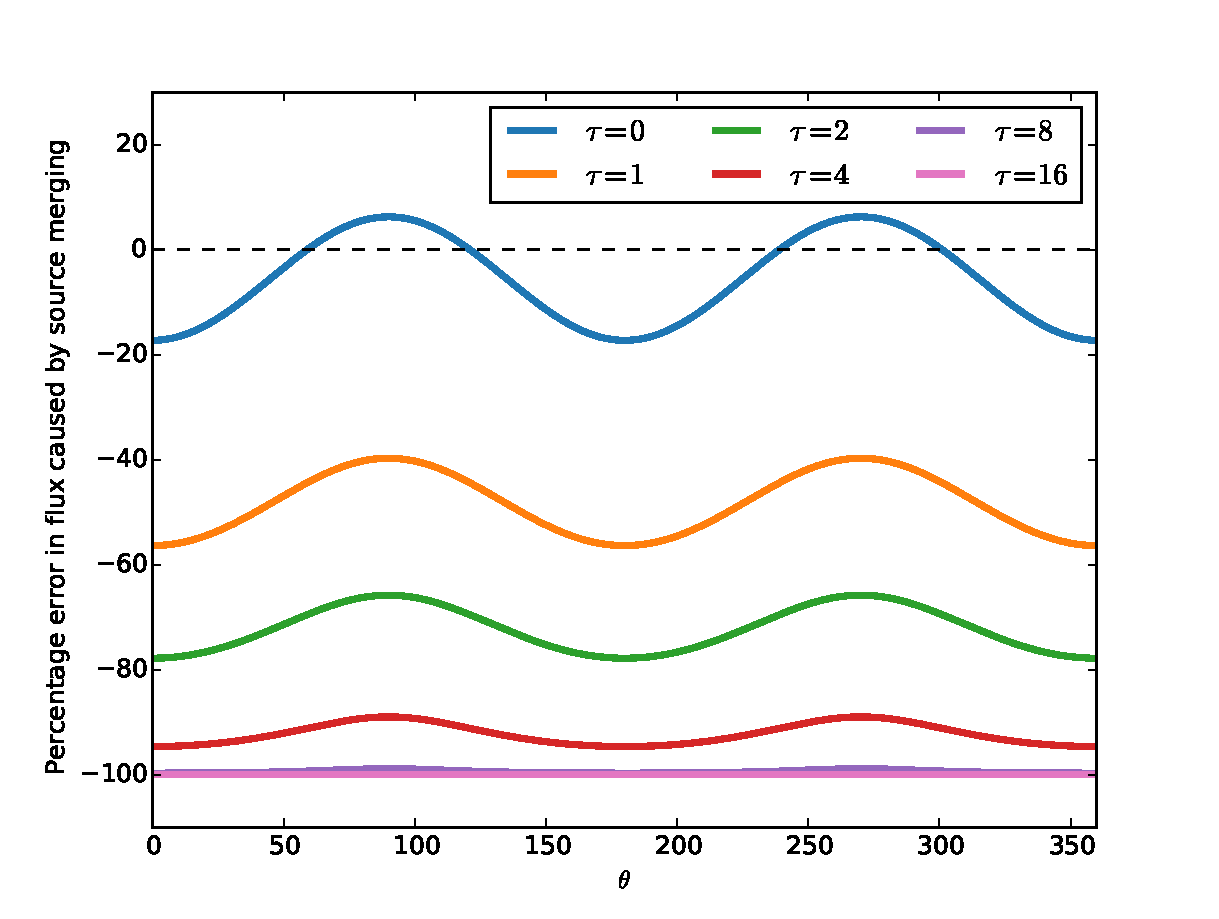
\includegraphics[width=\textwidth]{plots/CH4/CSError.pdf}
    \caption{Percentage error in flux due to source merging as a function of flux for varying optical depths}
    \label{fig:CSAngular}
\end{figure}

While the initial conditions used are simple, the systematic trend towards lower values for the flux when merging is what is expected in typical astrophysical set-ups where sources are embedded in absorbing material, this this suggests that this gives a reasonable toy model of real scenarios. Only scenarios such as sources merging into a region with a noticeably lower optical depth would cause systematic positive errors in the flux. This could occur but is less likely so we speculate that systematic reductions in flux are the most likely outcome.

The error in the flux caps at 100\% (i.e. $\sim$ 0 flux is received) at $\tau = 16$, with the plot suggesting that the error increases dramatically as one moves to higher optical depths. However, only looking at the percentage error doesn't take into account the absolute flux received by the sinks, shown in figure \ref{fig:CSAbsError}.

\begin{figure} [H]
    \centering
    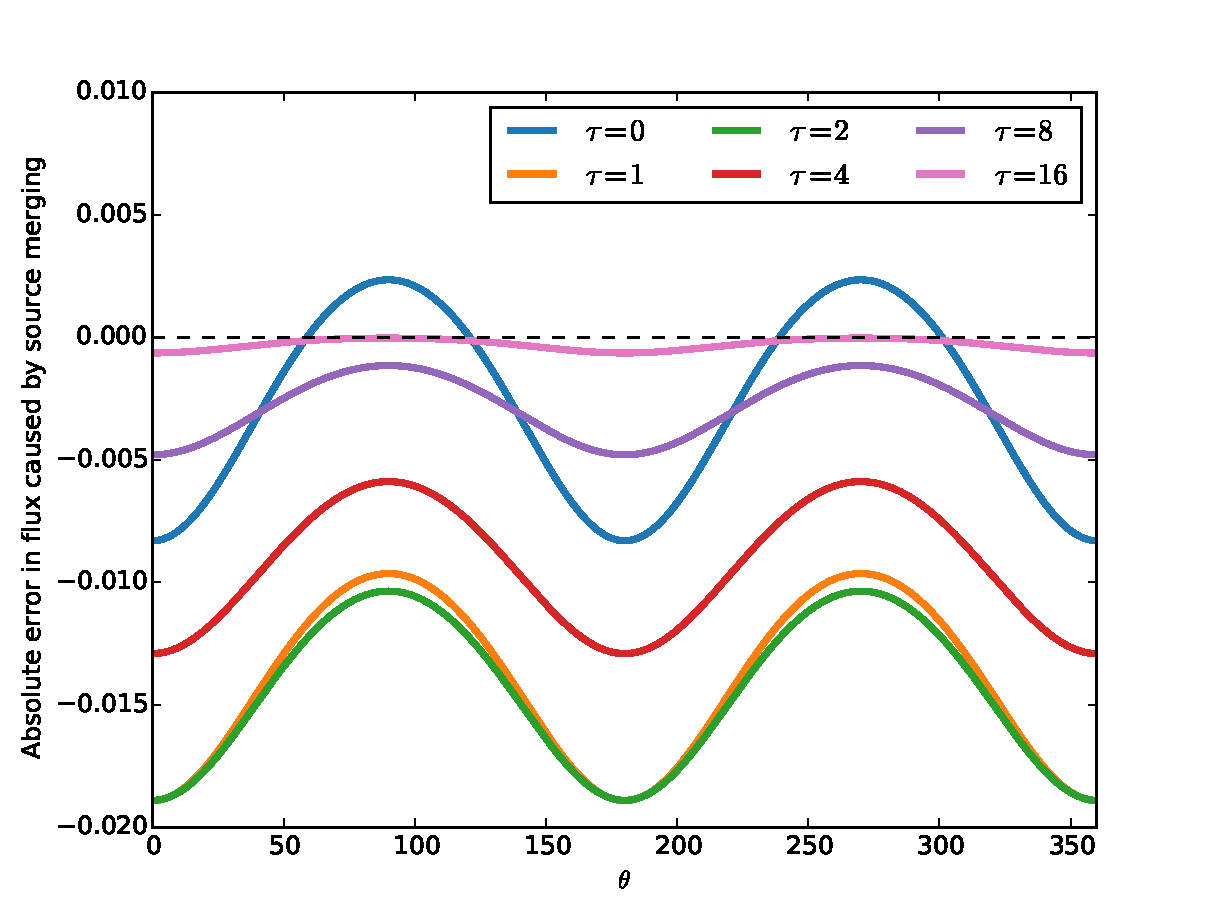
\includegraphics[width=\textwidth]{plots/CH4/CSAbsError.pdf}
    \caption{Absolute error in flux due to source merging as a function of flux for varying optical depths}
    \label{fig:CSAbsError}
\end{figure}

Of note is how the absolute error in the system peaks at approximately $\tau = 2$ before returning to approximately 0 at extreme values of $\tau$. This is due to the increase in optical depth reducing the magnitude of the flux able to escape the dense region resulting in a low absolute error regardless of the high percentage error. This suggests that regions with intermediate optical depths (order 1-2) suffer from the greatest error. Unfortunately, a large proportion of astrophysical systems fit into this category and thus makes solving the complex sources problem one of importance for accurately modelling radiation in astrophysical radiative transfer simulations.

\section{Resolving Complex Sources}

\subsection{Utilizing an Optical Depth Refinement Criterion}

The simplest approach is to implement a modification of the refinement criterion from the optically thick walk in the source walk. This would allow the source refinement to take into account the absorption properties of each node and only require minimal coding. Instead of looking at the optical depth differential, we instead take the distance that the child sources must move when merging and multiply it by the absorption coefficient for the node, giving the optical depth from source merging. If this optical depth is greater than a chosen refinement value, we refine on that node and all descendant nodes.
\iffalse
This was implemented into the tree build and ran on identical initial conditions to the opening angle tests shown in figure \ref{fig:openingTest}. A plot of the number of nodes flagged for refinement as a function of $\tau_{refine}$ is shown in fig \ref{fig:CSnumNodes}. The number of nodes flagged is comparable to the number of sources used and thus gives us an estimate of the cost.

\begin{figure} [H]
    \centering
    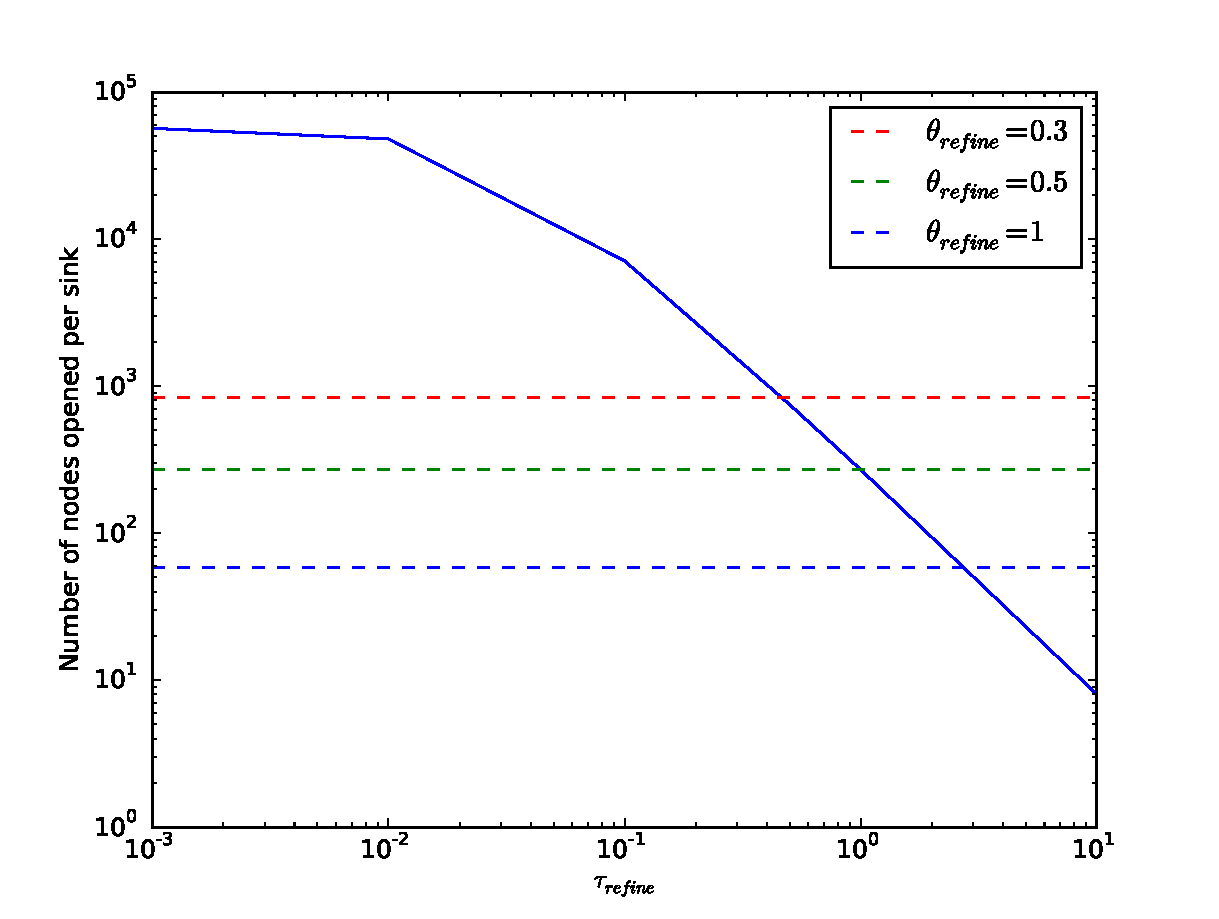
\includegraphics[width=\textwidth]{plots/CH4/CSOpeningTau.pdf}
    \caption{Number of tree nodes marked for refinement as a function of maximum perturbation in $\tau$ through a node with node opening counts of tree walks for $\theta_{refine}$ values of 0.3, 0.5 and 1 for comparison}
    \label{fig:CSnumNodes}
\end{figure}

It can be seen that utilizing a value for $\tau_{refine}$ similar to that used in the optically thick tree walk will result in substantially more nodes being opened, with approximately 2 orders of magnitude between our standard $\theta_{refine}$ value of 0.5 with no complex source refinement and the same with our standard $\tau_{refine}$ value of 0.01 used for complex source refinement.
\fi
As this method is only sensitive to the perturbation in the optical depth, it is of little use in scenarios such as those shown in figure \ref{fig:CSIC} where the density across the node is constant. As figures \ref{fig:CSAngular} and \ref{fig:CSAbsError} show, even constant density regions can cause large errors in the flux when merged. On the other hand, this method is excellent at finding cases where variations in the optical depth can cause the merged sources to drastically change the optical depth of the regions traced by the ray. This, combined with the method's low computational cost, suggests that this refinement criterion would work best when combined with others with each criterion working to eliminate a specific sub-type of complex source.

\subsection{Ray Tracing During Tree Build}

A more involved method for resolving the complex source problem is to utilize a simplified optically thick ray trace during the tree build that compares the variation in flux of combined (parent) and uncombined (child) sources to a sphere of background absorbers centred on the node, as shown in fig \ref{fig:CSrefExample}. The radius of this sphere should be set as equal to or greater than the distance that the node's sources would merge, calculated via equation \ref{eqn:openingTheta}. If the angular variation of the error in the calculated optical depths is too great, a variable in the parent node that tracks if precalculated refinement is necessary can be set to true. All nodes with this node as a descendant are also set to open without tracing. This results in every node refining to the first combined source that is deemed an accurate representation of their child nodes.

\begin{figure} [H]
    \centering
    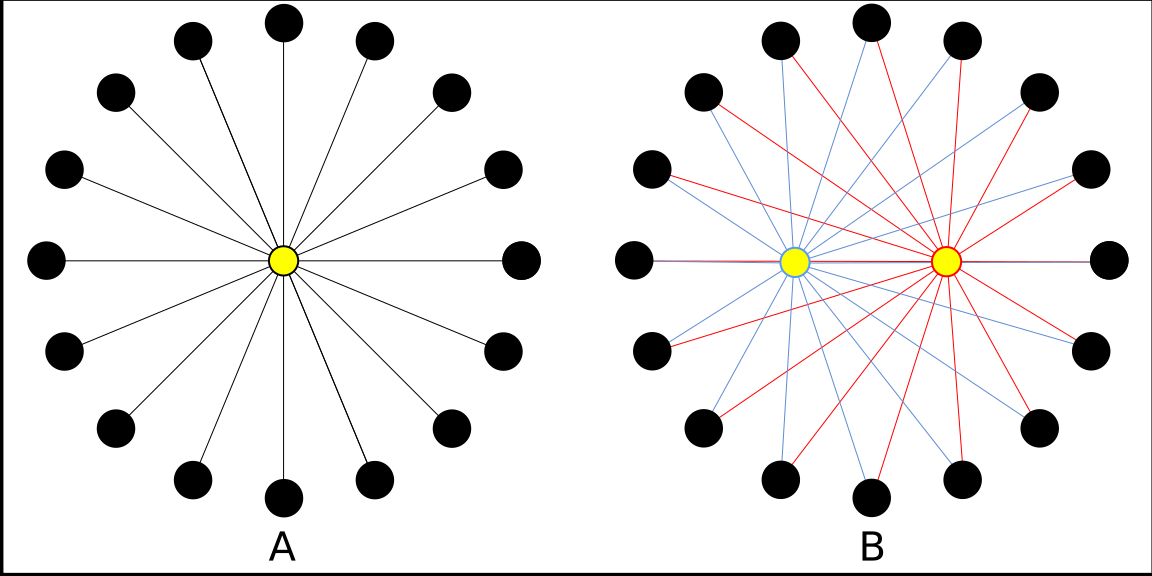
\includegraphics[width=\textwidth]{plots/CH4/CSDiagram.png}
    \caption{Diagram of the ray traces performed on parent (A) and child (B) nodes for the complex source refinement test during the tree walk}
    \label{fig:CSrefExample}
\end{figure}

Once this computation has been performed the refinement test during the tree walk can again be completed with minimal computational cost, only requiring a check to see if the node is flagged for refinement.

As each node will only have its centre of luminosity traced to a predetermined number of fake sinks, this method has a cost of only $\mathcal{O}(N)$ (where N is the number of nodes, which is proportional to the number of particles) but risks creating a scenario in which the reduction of computational cost given by the source walk opening criterion is nullified by the forced opening when complex sources are detected. 

This method can also be utilized for another purpose: direct flux correction. As figure \ref{fig:CSAbsError} clearly shows, there is a strong negative bias in the calculated flux when merging sources even for the optically thin case. By taking measurements of the error in the optically thin flux across the full sphere of the sky around the node, we can calculate an average flux bias and modify the absorption properties of each ray trace to mitigate this. This can be done by storing a correction factor that can be applied to each ray's calculated optical depth to account for the average flux loss due to source merging. Alternatively, a collection of values from a range of directions could be stored and the correction factor extrapolated from the combination of these values and the direction of the ray, although this would require more extensive data storage.

\subsection{Flux Tracking}

One method that can be used to reduce the cost of an increased sensitivity refinement criterion is flux tracking. This is where the total flux received by a sink is retained to the next timestep, allowing an estimate of the flux from each source to be calculated. If a source is estimated to contribute only a minor amount to the total flux, there is minimal benefit to fully resolving any complex sources. This relates to the fact, as shown in figure \ref{fig:CSAbsError} that the absolute error can be quite small for deeply embedded sources This allows for the added computational cost to be focused primarily on the sources with the greatest impact on the flux which keeps the total error bounded.

An alternative method is to use the optically thin flux of the sources from the current timestep and apply a optical depth estimator where the ray length is the euclidean distance between sink and source and the absorption coefficient is the averaged value for the entire box. All sources are found before commencing ray tracing and thus the total flux estimate can be calculated prior to the ray trace walk. The estimated contribution from each ray can then be compared to the total flux. This method can be combined with the optically thick refinement to help minimize its cost, although this would limit its ability to pre-calculate the refinement outcome during the tree build.

Care must be taken when applying this criterion due to the systematic negative error in the flux caused by merging. Any node that is merged will contribute to this error and thus applying this criterion without taking this into account will almost always increase this systematic error. Estimating a correction factor based on the the faction of the prior flux that the merged sources contributed could reduce this error but this risks forcing the total flux to remain at a constant value. Another option is to base the factor on the optically thin flux contribution estimate.

It should be noted that flux tracking can identify sources that are negligible regardless of complicating factors and which thus can be terminated. This technique could be applied to neglect even simple sources and save work. The challenge is to use a sufficiently conservative estimator to ensure the sources designated to be neglected are guaranteed to be small contributors. If the total flux is the product of many weak sources, then none of them can be neglected otherwise a systematic error is created. In addition, selecting a cruder representation (e.g. source merging) also requires care if the flux errors are systematic.
    
